%--
%-- Diagrama de Contexto
%--
\subsection{Diagrama de Contexto}

%--
%-- Agentes
%--
\subsubsection{Agentes}

\begin{enumerate}
  \item Depósito
  \item Cliente
  \item Sucursal
  \item Sistema
  \item Logística
  \item API de Logística
  \item Departamento de Stock
  \item Agente de Cobro
  \item Administrador
  \item Sistema de Correo Electrónico
  \item Financiera(API)\footnote{Ejemplo: VERAZ}
  \item Correo Argentino(API)
  \item Proveedor
\end{enumerate}
\clearpage

%--
%-- Listado de Fenómenos
%--

\subsubsection{Listado de Fenómenos}
\begin{enumerate}
  \item Configuración y uso por parte del Administrador
  \begin{enumerate}
    \item El Administrador define el umbral de redituabilidad en el Sistema \label{itm:f-administrador-umbral-sistema}
    \item El Administrador consulta estadísticas en el Sistema \label{itm:f-administrador-estadistica-sistema}
    \item El Administrador modifica producto a través de ABM \label{itm:f-administrador-modifica-productos}
  \end{enumerate}

  \item Registro presencial cliente
  \begin{enumerate}
    \item El Cliente presenta la documentación en la Sucursal \label{itm:f-cliente-documentacion-sucursal}
    \item El Cliente presenta la factura asociada al domicilio en la Sucursal \label{itm:f-cliente-domicilio-sucursal}
    \item El Cliente presenta datos de tarjeta en la Sucursal \label{itm:f-cliente-tarjeta-sucursal}
    \item La Sucursal presenta datos de tarjeta del cliente al Agente de Cobro \label{itm:f-sucursal-tarjeta-agentecobro}
    %\item El Agente de Cobro verifica la tarjeta de crédito del Cliente % no es interacción
    % \item La Sucursal verifica datos personales y de domicilio del Cliente % no es interacción
    \item La Sucursal carga datos del cliente en el Sistema \label{itm:f-sucursal-carga-cliente-sistema}
  \end{enumerate}

  \item Registro online cliente
  \begin{enumerate}
    \item El Cliente presenta datos de identificación personal y de domicilio al Sistema \label{itm:f-cliente-datos-personal-sistema}
    \item El Cliente presenta datos de pago al Sistema \label{itm:f-cliente-datos-pago-sistema}
    \item El Sistema valida domicilio con el Correo Argentino \label{itm:f-sistema-valida-correoargentino}
    \item El Sistema evalúa estado financiero del cliente con la Financiera. \label{itm:f-sistema-evalua-financiera}
    \item El Sistema le indica al Correo Electrónico que envíe mail de confirmación al Cliente. \label{itm:f-sistema-confirmacion-correoelectronico}
    %\item El Sistema añade al Cliente.
    \fixme[poner que sist. pide validacion de datos de pago a agente de cobro, y la vuelta]
  \end{enumerate}

  \item Armado carrito
  \begin{enumerate}
    \item El Cliente ingresa credenciales en el Sistema \label{itm:f-cliente-autentica-sistema}
    \item El Sistema muestra stock disponible al Cliente \label{itm:f-sistema-muestra-stock-cliente}
    \item El Sistema muestra recomendaciones al Cliente \label{itm:f-sistema-muestra-recomendaciones-cliente}
    \item El Cliente selecciona mercadería en el Sistema \label{itm:f-cliente-elige-mercaderia-sistema}
  \end{enumerate}

\item Confirmación compra
  \begin{enumerate}
    \item Cliente confirma carrito al sistema \label{itm:f-cliente-confirma-carrito-sistema}
    \item Sistema ratifica al cliente stock disponible \label{itm:f-sistema-confirma-stock-cliente}
    \item Sistema muestra mensaje de error de producto no disponible al cliente \label{itm:f-sistema-error-stock-cliente}
    \item El sistema obtiene el costo del envío de la API de Logística \label{itm:f-apilogistica-envia-costo-sistema}
    \item El sistema informa el costo de la compra y el envío al cliente \label{itm:f-sistema-envia-costo-cliente}
    \item El sistema pregunta próximas fechas libres a la API de logística \label{itm:f-apilogistica-fechas-libres-sistema}
    \item El sistema presenta las posibles fechas de entrega al cliente \label{itm:f-sistema-fechas-libres-cliente}
    \item El cliente indica la fecha de entrega deseada al sistema \label{itm:f-cliente-fecha-entrega-sistema}
    \item El sistema presenta los métodos de pago disponibles al cliente \label{itm:f-sistema-muestra-metodos-pago-cliente}
    \item El cliente elige el método de pago \label{itm:f-cliente-elige-metodo-pago-sistema}
    \item El sistema muestra datos de pago asociados al cliente \label{itm:f-sistema-muestra-datos-pago-cliente}
    \item El cliente indica dato de pago \label{itm:f-cliente-elige-dato-pago-sistema}
    \item El sistema redirige al cliente a la ventana del Agente de Cobro \label{itm:f-sistema-redirige-cliente}
    \item El cliente autoriza la operación en la ventana del Agente de Cobro \label{itm:f-cliente-autoriza-agentecobro}
    \item El agente de cobro envía estado y comprobante al sistema \label{itm:f-agentecobro-comprobante-sistema}
    \item El sistema pide mail de comprobante de pago al Correo Electrónico \label{itm:f-sistema-envia-comprobante-correoelectronico}
    \item El sistema informa de error de pago al cliente \label{itm:f-sistema-error-pago-cliente}
    \item El sistema muestra error de timeout de carrito al cliente \label{itm:f-sistema-error-timeout-cliente}
    \item El Sistema ofrece pago de multa al cliente \label{itm:f-sistema-ofrece-multa-cliente}
    \item El cliente paga multa online (mediante agente de cobro) \label{itm:f-cliente-paga-multa-agentecobro}
    \item El cliente paga multa en efectivo a logística \label{itm:f-cliente-paga-multa-logistica}
  \end{enumerate}

\item Modificación de pedido
  \begin{enumerate}
    \item El Cliente modifica un pedido no cerrado en el Sistema \label{itm:f-cliente-modifica-pedido-sistema}
    \item El Sistema le da un crédito al Cliente si este quita mercadería paga \label{itm:f-sistema-da-credito-cliente}
  \end{enumerate}

\item Preparación y entrega
  \begin{enumerate}
    \item El Cliente confirma el pedido al Sistema \label{itm:f-cliente-confirma-pedido-sistema}
    \item El Sistema avisa al Depósito que prepare el pedido \label{itm:f-sistema-avisa-pedido-deposito}
    \item El Depósito informa egreso de mercadería al Departamento de stock \label{itm:f-sistema-egresa-mercaderia-dptostock}
    \item El Depósito avisa al Sistema que el pedido está cerrado \label{itm:f-deposito-cerro-pedido-sistema}
    \item El Depósito entrega mercadería a Logística \label{itm:f-deposito-entrega-mercaderia-logistica}
    \item Si forma de pago es contraentrega:
    \begin{enumerate}
      \item Cliente paga el pedido a Logística \label{itm:f-cliente-paga-logistica}
    \end{enumerate}
    \item Logística entrega el pedido al Cliente \label{itm:f-logistica-entrega-cliente}
    % \item El Sistema actualiza positivamente el perfil del Cliente % operacion interna del sistema
  \end{enumerate}

\item Entrega fallida
  \begin{enumerate}
    \item El Cliente no recibe pedido a Logística \label{itm:f-cliente-no-recibe-logistica}
    \item Si el pedido fue pagado:
    \begin{enumerate}
      \item El Sistema le envía una nota de crédito como reintegro del pedido al Agente de Cobro. \label{itm:f-sistema-reintegra-agentecobro}
      \item Agente de Cobro genera el comprobante de reintegro y se la envía al Sistema. \label{itm:f-agentecobro-comprobante-reintegro-sistema}
      \item El Sistema envía el comprobante al Cliente. \label{itm:f-sistema-comprobante-reintegro-cliente}
    \end{enumerate}

    % \item El Sistema añade una no-recepción al historial de recepciones del Cliente % operacio interna del sistema
    \item Logística devuelve el stock al Depósito \label{itm:f-logistica-devuelve-stock-deposito}
    % \item El Sistema genera un link al pedido fallado.
    \item El Sistema arma un e-mail con el link al pedido fallido y la propuesta para que el cliente lo vuelva a hacer, y se lo envía al Sistema de Correo \label{itm:f-sistema-link-rehacer-correoelectronico}
    \item El Sistema de Correo electrónico envía mail al Cliente. \label{itm:correoelectronico-mail-cliente}
  \end{enumerate}

\item Reposición stock sucursal
  \begin{enumerate}
    \item La Sucursal avisa cuando falta stock al Sistema \label{itm:f-sucursal-falta-stock-sistema}
    \item El Sistema avisa falta de stock en sucursal al Depósito \label{itm:f-sistema-falta-stock-deposito}
    \item El Depósito arma pedido y entrega el stock a Logística \label{itm:f-deposito-entrega-pedido-logistica}
    \item El Sistema disminuye stock en el Depósito \label{itm:f-sistema-disminuye-stock-deposito}
    \item Logística entrega stock a la Sucursal \label{itm:f-logistica-entrega-stock-sucursal}
  \end{enumerate}

\item Reposición stock deposito
  \begin{enumerate}
    \item El Departamento de stock modifica los límite mínimos de stock estipulado para cada producto en el Sistema \label{itm:f-deptostock-limite-stock-sistema}
    \item El Sistema avisa que hay faltante de producto al Departamento de stock \label{itm:f-sistema-falta-producto-deptostock}
    \item El Departamento de stock encarga reposición de stock del depósito a Logística \label{itm:f-deptostock-encarga-stock-logistica}
    \item Logística repone stock al Depósito \label{itm:f-logistica-repone-stock-deposito}
  \end{enumerate}

\end{enumerate}
\clearpage

%--
%-- Acciones Básicas
%--
\subsubsection{Diagrama de Contexto}

\begin{figure}[H]
  \begin{center}
  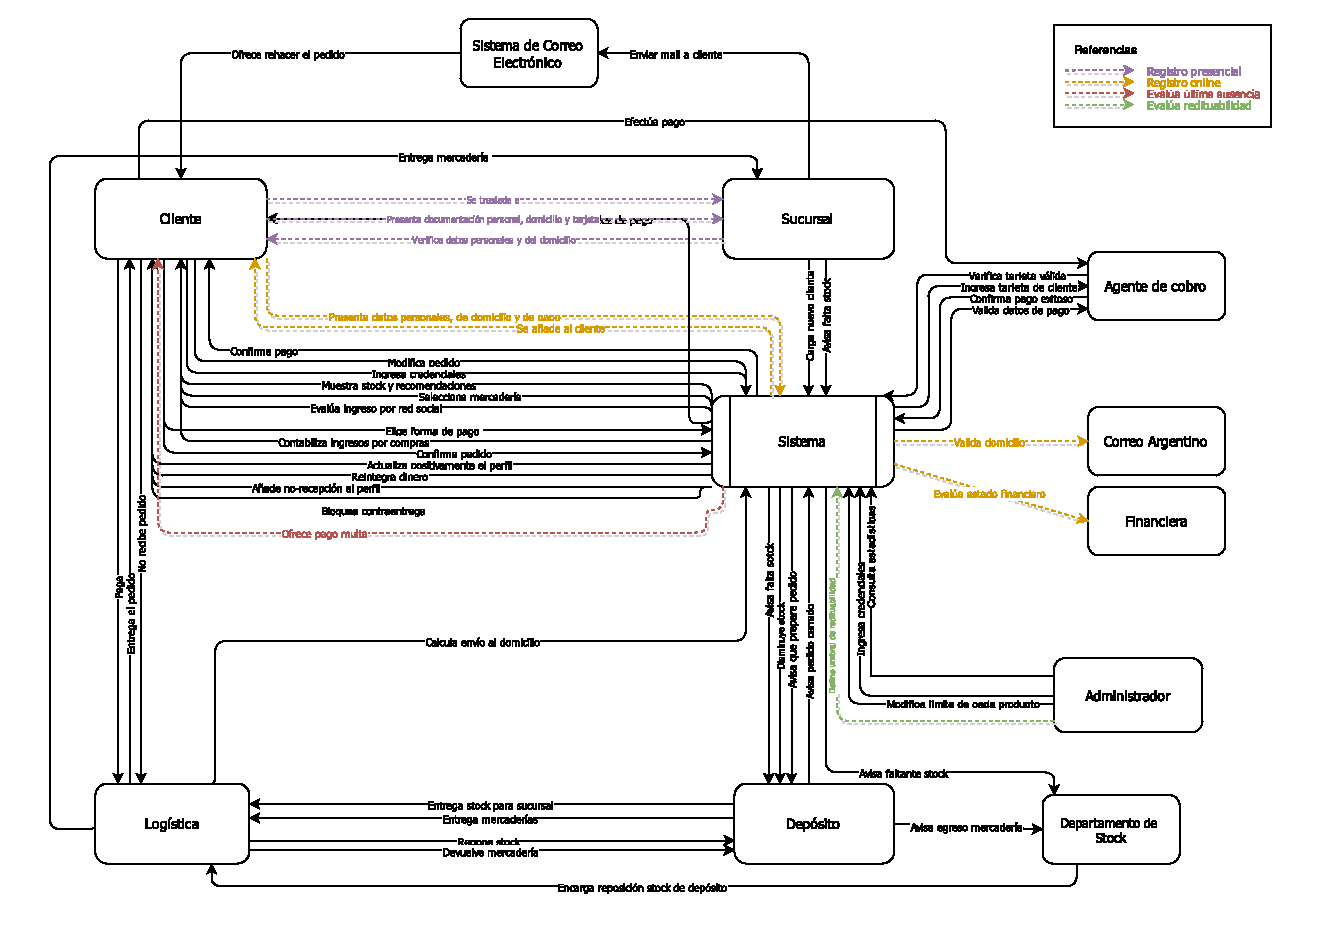
\includegraphics[height=0.65\textheight,angle=90]{tp1/images/contexto.pdf}
  \end{center}
\end{figure}
